\documentclass[11pt, quiet, fontset = fandol]{ctexart}

\usepackage{hyperref, xeCJKfntef, menukeys, hologo, fancyhdr,
            tikz, subcaption, pgfmorepages, twemojis}
\hypersetup{hidelinks}
\usepackage[mono = false]{libertine}
\usepackage[margin = 1in, headheight = 13.6pt]{geometry}
\graphicspath{{./figures/}}
\pagestyle{empty}
\def\UrlFont{\tt\color{red}}
\newcommand*\sh \texttt
\newcommand*\pkg \texttt
\newcommand*\file \texttt
\let \emph \textbf
\makeatletter \def \HoLogo@CTeX #1{\HOLOGO@mbox {C\TeX}} \makeatother

\begin{document}

\pgfmorepagesloadextralayouts
\pgfpagesuselayout{2 on 1}
\pagestyle{fancy} \let \headrule \relax \cfoot{}
\rfoot{\color{gray}%
  Remade by \href{https://github.com/myhsia}{\ttfamily @myhsia}}

\section*{有这么多的截图键\ldots}

\begin{figure}[htbp]
  \begin{subfigure}{.48\linewidth}
    \centering
    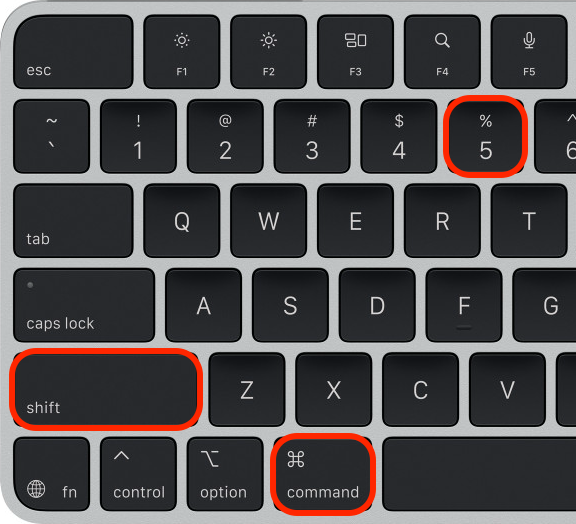
\includegraphics[height = .48\linewidth]{macOS}\hspace{-3.33pt}
    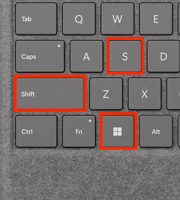
\includegraphics[height = .48\linewidth]{Windows}
    \caption{乔帮主 / 盖茨给你的截图键}
  \end{subfigure}
  \hspace*{\fill}
  \begin{subfigure}{.48\linewidth}
    \centering
    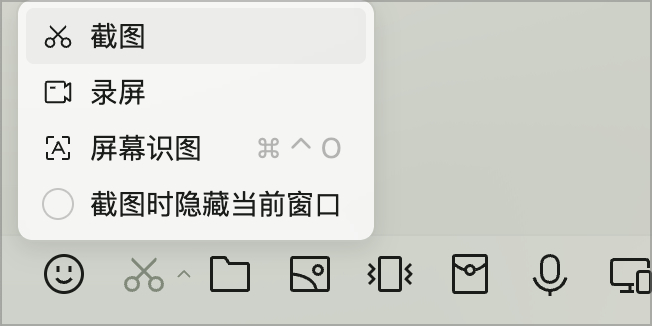
\includegraphics[width = .96\linewidth]{QQ}
    \caption{化腾给你的截图键}
  \end{subfigure}
  \begin{subfigure}{.48\linewidth}
    \centering
    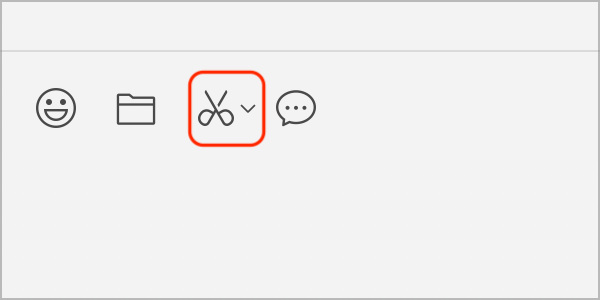
\includegraphics[width = .96\linewidth]{WeChat}
    \caption{小龙给你的截图键}
  \end{subfigure}
  \hspace*{\fill}
  \begin{subfigure}{.48\linewidth}
    \centering
    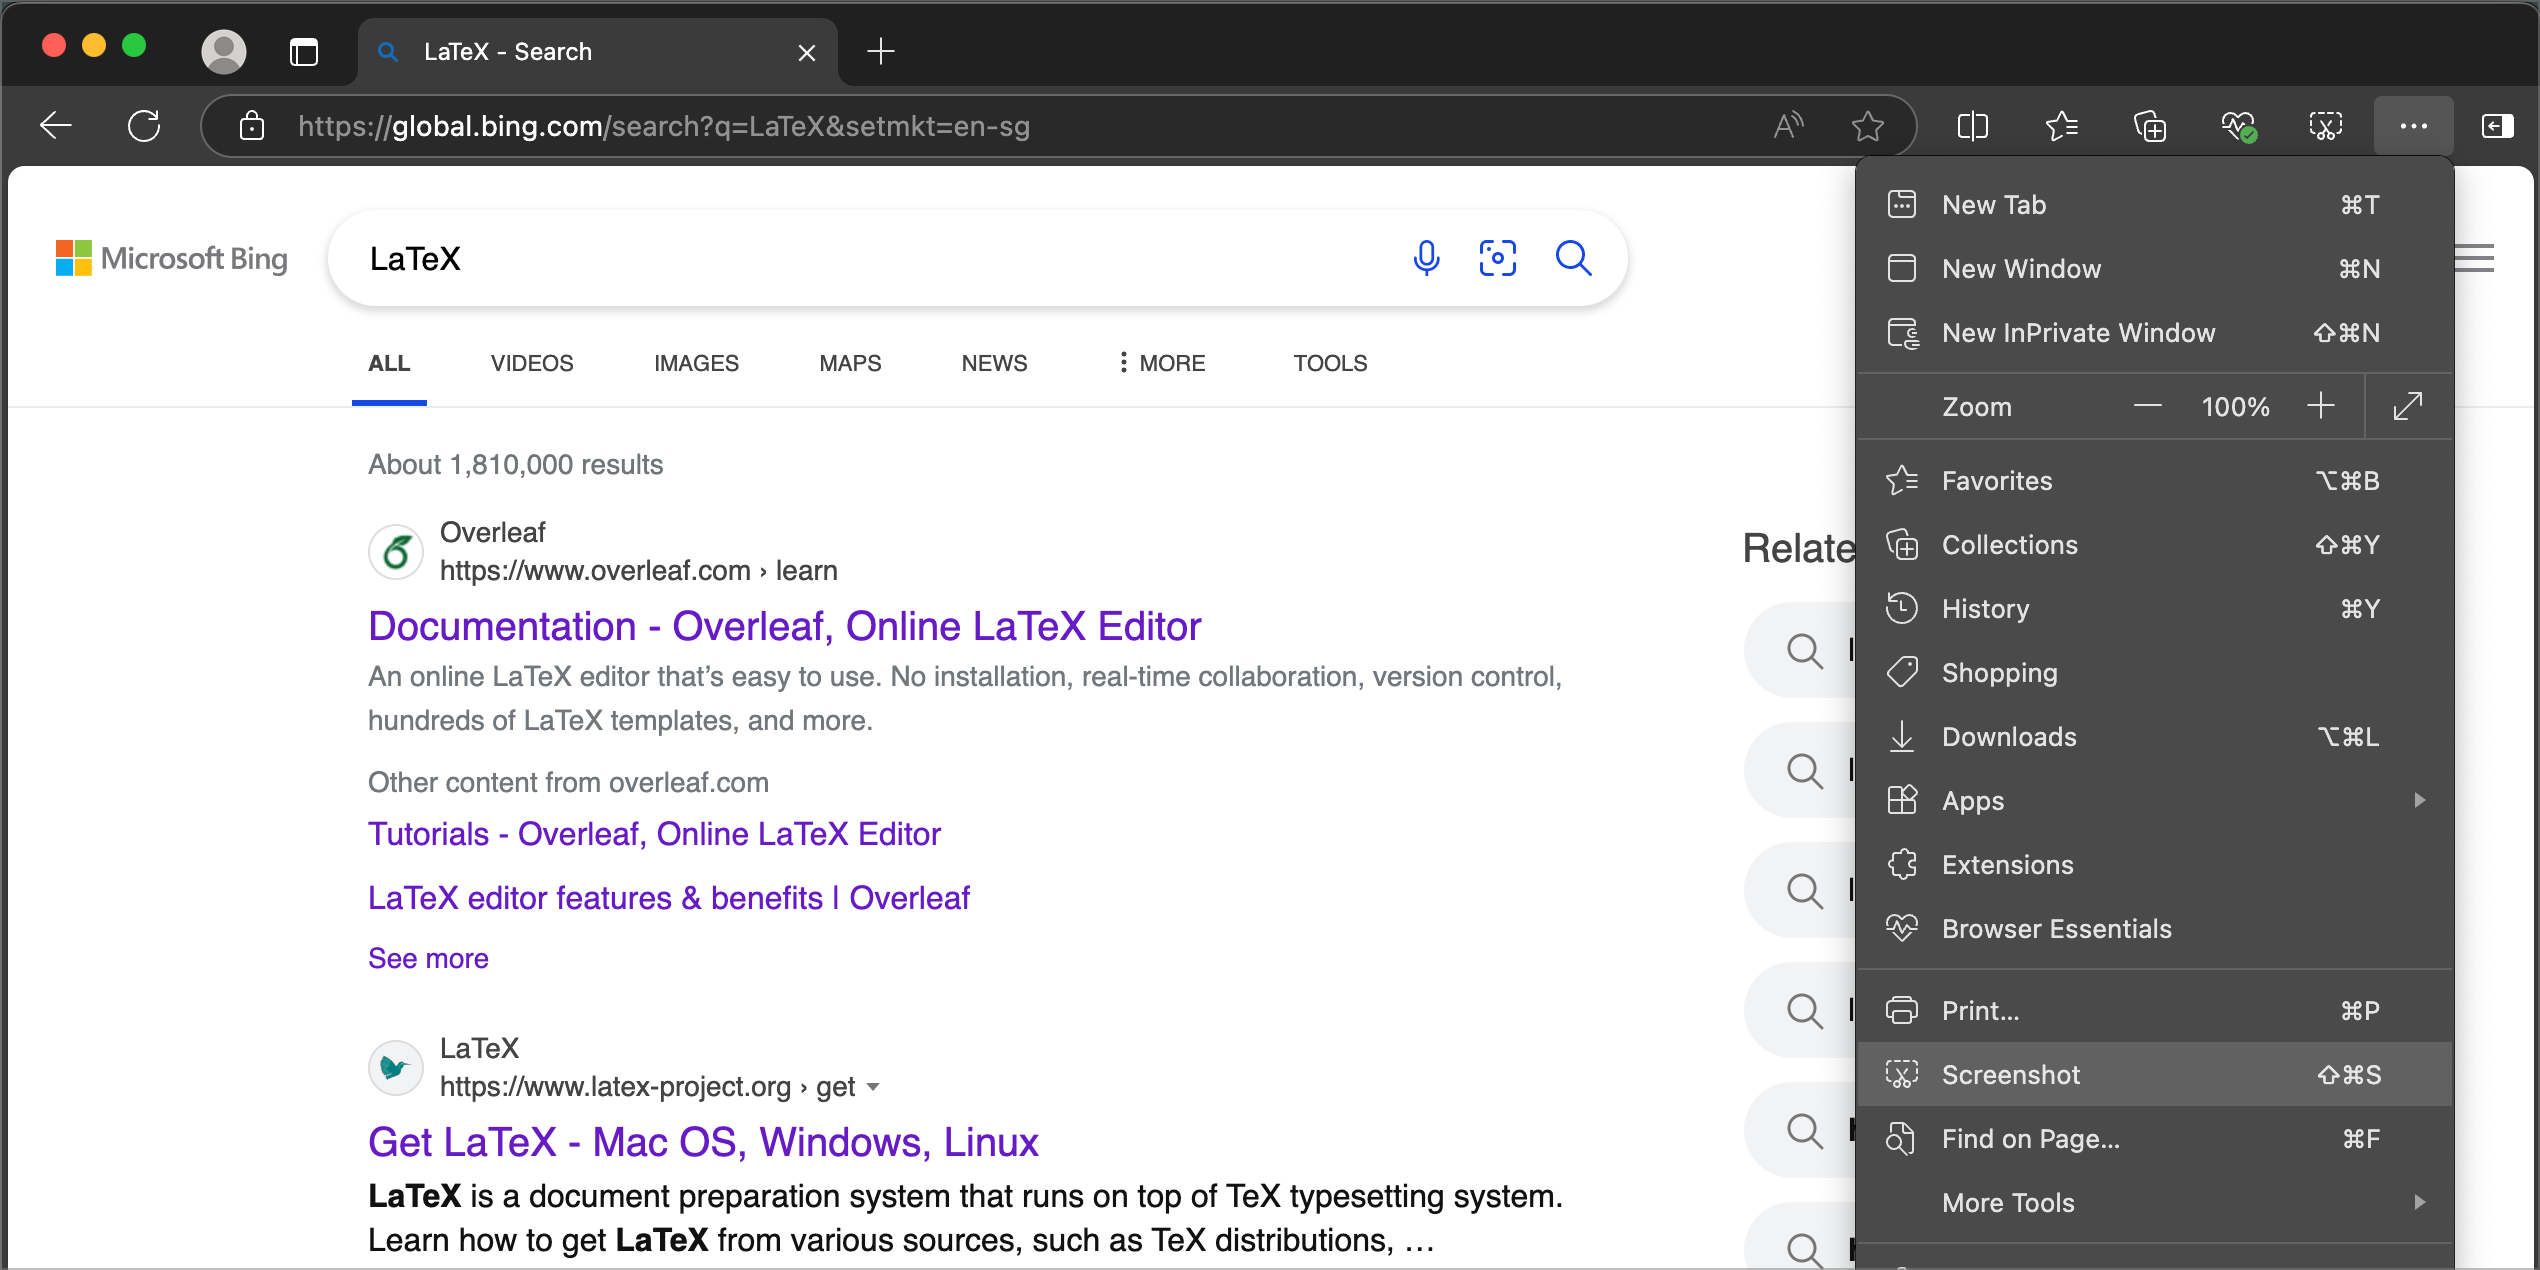
\includegraphics[width = .96\linewidth]{Edge}
    \caption{Edge 自带的截图键}
  \end{subfigure}
  \begin{subfigure}{.48\linewidth}
    \centering
    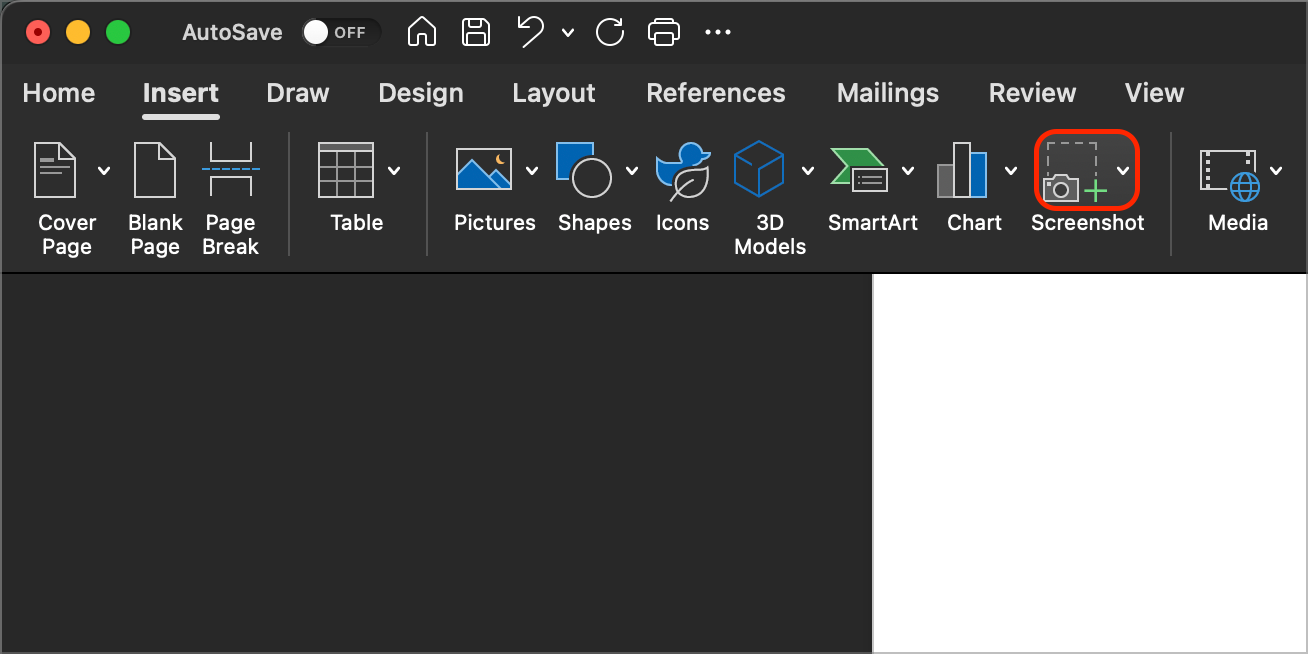
\includegraphics[width = .96\linewidth]{Office}
    \caption{Office 自带的截图键[请顺带卸载你的 WPS]}
  \end{subfigure}
  \hspace*{\fill}
  \begin{subfigure}{.48\linewidth}
    \begin{itemize}
      \item \menu{ctrl > print}:截取整个屏幕
      \item \menu{ctrl > alt > print}:截取指定窗口
      \item \menu{ctrl > shift > print}:截取指定区域
    \end{itemize}
    \caption{Ubuntu 给你的截图键}
  \end{subfigure}
\end{figure}

\section*{\ldots 但总有人想展示 Ta 的拍照技术}

\begin{center}
  \begin{minipage}{.64\linewidth}
    \tikz
      {
        \node [ scale = 9.6, inner sep = 0pt ] (sweat) {\twemoji{1f605}};
        \node [ right, align = center, scale = 2.4, font = \bfseries ]
          at (sweat.east) {仍然没有学会截图\\ NewBee};
      }
    
    右图这种\emph{伤害大家视力}的行为,管理员看见后会直接撤回,丝毫不会手下留情.
    建议意识到后\emph{主动撤回}.
  \end{minipage}
  \hspace*{\fill}
  \begin{minipage}{.32\linewidth}
    \raggedleft
    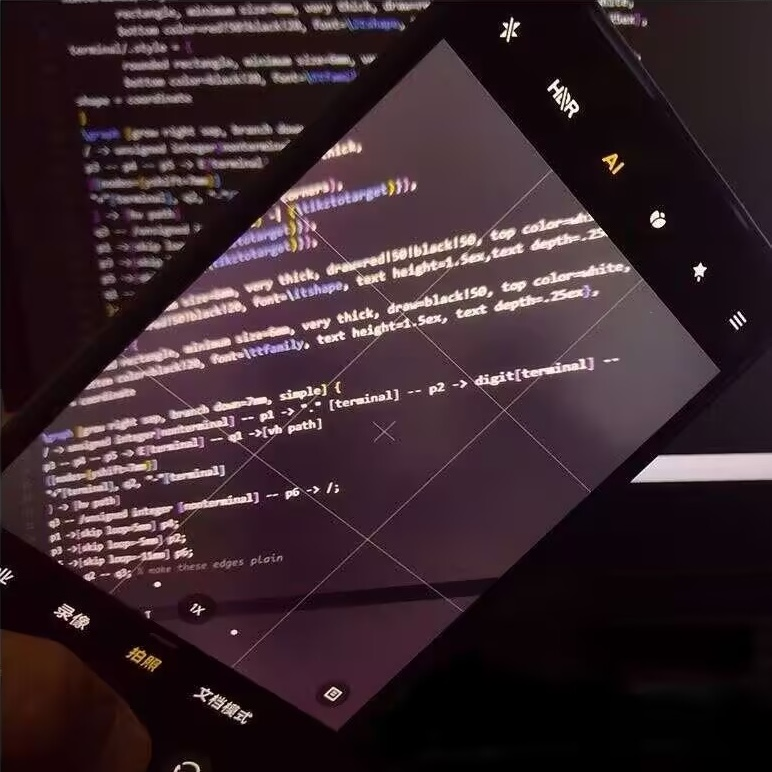
\includegraphics[height = .9\linewidth]{photo}
  \end{minipage}
\end{center}

\newpage

\section*{\hologo{LaTeX} 交流提问的艺术:从学会制作 MWE 开始}

编译出错,效果不满意,想得到有针对性地帮助,请提供\emph{最小工作示例代码}%
(\emph Minimal \emph Working \emph Example, \emph{MWE}),
完整 MWE 包括以下信息:
\begin{enumerate}
  \item 你使用的\emph{操作系统}(Windows 7/10/11,macOS,Ubuntu,Deepin 等).
  \item 安装的\emph{发行版}
    (\hologo{TeX} Live 2025,Mac\hologo{TeX},
      \hologo{MiKTeX},\hologo{CTeX} 套装).
  \item 你使用的\emph{编辑器}
    (TeXstudio,Visual Studio Code,WinEdt,TeXshop,Overleaf).
  \item 你执行的\emph{编译命令}及\emph{编译顺序}
    (\sh{latex},\sh{pdflatex},\sh{xelatex},\sh{latexmk},\sh{bibtex},
      \sh{biber}等),或者点击编辑器图形界面上的按钮.
  \item 最重要的一点:
  \CJKunderline[textformat = \bfseries]{直接复制粘贴上能复现你问题的}%
  \footnote{如果没有特殊需求,禁止使用 \hologo{CTeX} 套装,它已经完成了历史使命,
    请换用现代的 \hologo{LaTeX} 发行版},
  \CJKunderline[textformat = \bfseries]{体量最小的}%
  \footnote{如果文档内容涉密,
    文字内容请使用 \pkg{lipsum} 和(或) \pkg{zhlipsum} 宏包生成随机乱数假文,
    图片请使用 \file{example-image} 代替,参考文献请使用 \file{xampl.bib} 代替,
    详细信息可见 \pkg{mwe} 宏包的说明文档(命令行执行 \sh{texdoc mwe} 获取).%
  },
  \CJKunderline[textformat = \bfseries]{可编译的示例代码的文本}%
  \footnote{请尽量使用最新版的模板,使用模板之前请先仔细阅读模板的使用说明.}.
  \begin{enumerate}
    \item 提供的代码需要复现你的问题,不要发一套代码,说另一套效果.
    \item 删除所有与问题无关的宏包引入命令,与问题无关的冗长代码,仅保留会出现问题的宏包与文本.
    \item 从 \verb|\documentclass{}| 开始,到 \verb|\end{document}| 结束.
    \item 效果可截图,但\emph{源代码不要截图!\textcolor{red}{不要拍屏幕!}}%
    \footnote{Windows / macOS / Ubuntu 等系统均有截图工具. 在交流群中拍屏提问者,
      管理员有权直接撤回.}
    使潜在的帮助者可以直接复制代码到他们自己编辑器中,编译报同样的错,节省大家的时间.
    \item 代码很长,建议发在 \url{https://pastecode.dev} 再提供链接;代码简短,可直接复制粘贴. 涉及文件过多,也可打包 \file{.zip} 或 \file{.tar.gz} 文件.
  \end{enumerate}
  \item 如实现某种需求,请\emph{明确}提供该需求的\emph{来源},需求的必要环境(如要使用在列表环境内,必须使用 \file{xelatex} 编译等等).
  \item 可以截图提供错误信息,奇怪的输出效果,可以通过 PS 等手段制作出你想要实现的效果图.
  \item 如果使用\emph{模板}。请提供模板文件(\file{.cls},\file{.sty}),或提供模板文件的获取方式.
  \item 一般更建议将以上信息发布到论坛%
  \footnote{如 \url{https://ask.latexstudio.net}, \url{https://tex.stackexchange.com}, \url{https://github.com/CTeX-org/forum/issues}}
  中.
  \item \emph{如果无法主动提供信息,请明确说明并且及时回复潜在帮助者的提问.}
\end{enumerate}


\end{document}